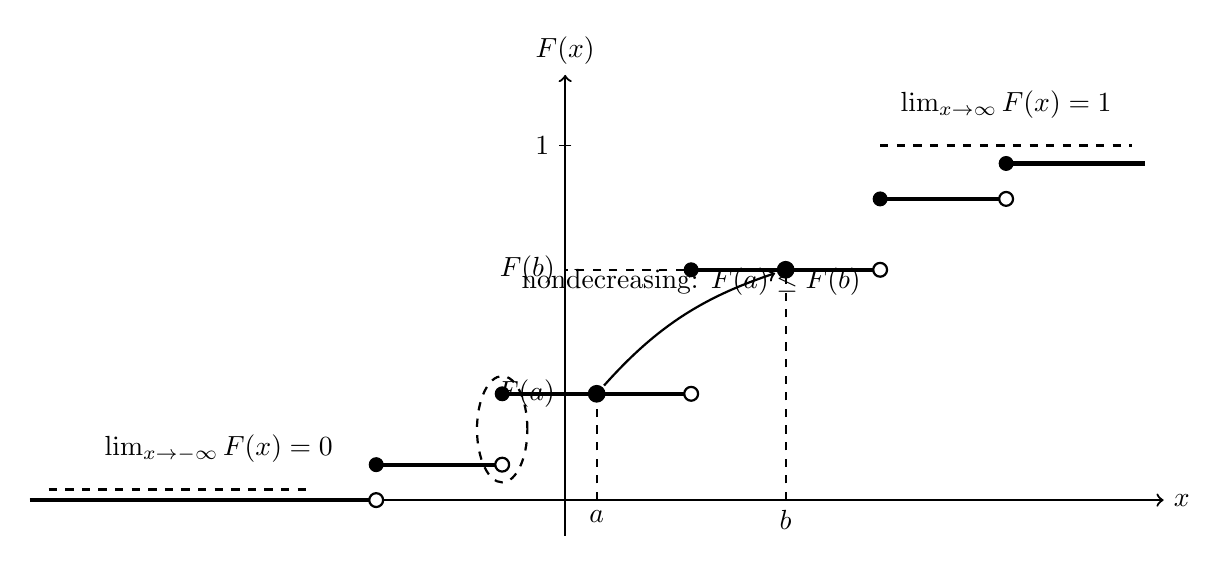
\begin{tikzpicture}[x=0.8cm, y=4.5cm]

\gid{axes}{
    \draw[->, thick] (-8.5, 0) -- (9.5, 0) node[right] {$x$};
    \draw[->, thick] (0, -0.1) -- (0, 1.2) node[above] {$F(x)$};
    \draw (0.1, 1) -- (-0.1, 1) node[left] {$1$};
}

\gid{asymptote-left}{
    \draw[dashed, line width=1.2pt] (-8.2, 0.03) -- (-4, 0.03);
}

\gid{label-limit-left}{
    \node[above] at (-5.5, 0.08) {$\lim_{x \to -\infty} F(x) = 0$};
}

\gid{asymptote-right}{
    \draw[dashed, line width=1.2pt] (5, 1) -- (9, 1);
}

\gid{label-limit-right}{
    \node[above] at (7, 1.05) {$\lim_{x \to \infty} F(x) = 1$};
}

\gid{cdf-curve}{
    % x < -3
    \draw[line width=1.5pt] (-8.5, 0) -- (-3, 0);
    \filldraw[white, draw=black, thick] (-3, 0) circle (2.5pt);
    
    % -3 to -1
    \filldraw[black] (-3, 0.1) circle (2.5pt);
    \draw[line width=1.5pt] (-3, 0.1) -- (-1, 0.1);
    \filldraw[white, draw=black, thick] (-1, 0.1) circle (2.5pt);
    
    % -1 to 2
    \filldraw[black] (-1, 0.3) circle (2.5pt);
    \draw[line width=1.5pt] (-1, 0.3) -- (2, 0.3);
    \filldraw[white, draw=black, thick] (2, 0.3) circle (2.5pt);
    
    % 2 to 5
    \filldraw[black] (2, 0.65) circle (2.5pt);
    \draw[line width=1.5pt] (2, 0.65) -- (5, 0.65);
    \filldraw[white, draw=black, thick] (5, 0.65) circle (2.5pt);
    
    % 5 to 7
    \filldraw[black] (5, 0.85) circle (2.5pt);
    \draw[line width=1.5pt] (5, 0.85) -- (7, 0.85);
    \filldraw[white, draw=black, thick] (7, 0.85) circle (2.5pt);
    
    % 7 to >7
    \filldraw[black] (7, 0.95) circle (2.5pt);
    \draw[line width=1.5pt] (7, 0.95) -- (9.2, 0.95);
}

\gid{marker-a}{
    \draw[dashed, thick] (0.5, 0) node[below] {$a$} -- (0.5, 0.3) -- (0, 0.3) node[left] {$F(a)$};
    \filldraw[black] (0.5, 0.3) circle (3pt);
}

\gid{marker-b}{
    \draw[dashed, thick] (3.5, 0) node[below] {$b$} -- (3.5, 0.65) -- (0, 0.65) node[left] {$F(b)$};
    \filldraw[black] (3.5, 0.65) circle (3pt);
}

\gid{label-monotone}{
    \draw[->, thick, shorten >=4pt, shorten <=4pt] (0.5, 0.3) to[bend left=15] (3.5, 0.65);
    \node[above] at (2, 0.55) {nondecreasing: $F(a) \le F(b)$};
}

\gid{jump-marker}{
    \draw[thick, dashed] (-1, 0.2) ellipse [x radius=0.4, y radius=0.15];
}

\end{tikzpicture}